\documentclass[12pt, a4paper]{article}

\usepackage{graphicx}


\date{24 Dicembre 2019}
\title{Riassunto}
\author{Psicobiologia}




\begin{document}

\maketitle

\newpage

\tableofcontents

\newpage

\section{Propriocezione}

Ci sono diverse rappresentazioni corporee: 

\paragraph{L'immagine corporea}  corrisponde all'uso quotidiano del termine, è una rappresentazione cosciente del corpo come visto frontalmente da un osservatore esterno

\subsection{Lo schema corporeo}  
È utilizzato per coordinare ed adattare i movimenti in base alla posizione del corpo, è una rappresentazione posturale incosciente che possiede 7 proprietà:

\subparagraph{Codifica Spaziale} 

L'oggetto dello schema corporeo è rappresentato in avente una posizione nello spazio con un volume da esso occupato.
\medskip\\ 
Integra l'informazione tattile con quella propriocettiva, permettendo di localizzare il corpo nel mondo esterno. Generalmente la localizzazione somatotopica e spaziale coincidono, ma non sempre, e in quei casi siamo più lenti ad elaborare.

\subparagraph{Modularità} Unghie appartengono a dita che appartengono a mani che appartengono a braccio ecc\ldots

\subparagraph{Aggiornamento con il movimento} Lo schema corporeo si modifica con il movimento, e si hanno dei neuroni che rispondono a stimoli visivi collocati dove si rappresenta un pezzo di corpo.

\subparagraph{Adattabilità} Si adatta ai cambiamenti ontogenetici (arto artificiale, manca termoregolazione nell'arto reale e aumenta autoimmunità). Si adatta anche ai cambiamenti filogenetici.
\subparagraph{Supramodalità} Interazione tra diverse modalità sensoriali, tra elaborazione superiore e primaria.
\subparagraph{Coerenza} È necessario mantenere coerenza (illusione di Pinocchio).
\subparagraph{Interpersonalità} Lo schema corporeo è utilizzato per comprendere posture altrui (+ attivazione braccio + riconoscimento postura braccio).


\subsection{Le rappresentazioni corticali}

Ci sono rappresentazioni di basso livello punto-punto, poi gli homunculus sensoriali e motori con estensione proporzionale all'innervazione, mappe superiori intermodali e supramodali.

Distretti coinvolti:

\begin{itemize}
    \item S1 afferenze controlaterali
    \item S2 afferenze bilaterali
    \item Corteccia premotoria
    \item Corteccia motoria
    \item Insula consapevolezza enterocettiva, stati interni del corpo
\end{itemize}

Network definito \emph{matrice corporea corticale}, offre appartenenza, protezio\-ne psico e fisiologica (insula ha proiezioni discendenti e regolano funzioni fisiologiche di base)

\subsection{Disturbi dello schema corporeo}

\paragraph{Arto fantasma e telescoping} Interpretato come riorganizzazione delle aree circostanti, che anche prima ricevevano afferenze da quelle aree ma erano inibite.

\paragraph{Arti sovrannumerari} Stimolazione degli arti reali produce effetti inferiori in S2 ma non in S1 quando l'arto fantasma è presente.
Una possibile spiegazione è che ci ofsse un deficit di integrazione tra comandi motori e feedback (muovo il braccio ma non mi sembra si sia mosso x disconnessione emisferica e danno frontale, quindi ho un braccio un più).
Anche questa percezione è riproducibile illusoriamente

\paragraph{Fading limbs}  Lesione parietale sinistra \emph{senza neglect}: se non osservo il braccio scompare.

\paragraph{Micro e macrosomatoagnosia}  Percezione legata a disturbi (epilessia, emicrania) dell'intero corpo come più piccolo o più grande, o anche di una mano e distretti limitrofi nell'homunculus come più grandi in seguito ad anestesia $\rightarrow$ importanza afferenze nella rappresentazione.

\paragraph{Sindrome di Alice in Wonderland} micro e macrosomatoagnosia in età evolutiva conseguente ad emicranee e epilessia, detta anche di Todd.

\paragraph{Somatoparafrenia}  associata a neglect e anosoagnosia, spesso correlata a lesione destre estese: deficit dell'integrazione multisensoriale.

\paragraph{Body Integrity Identity Disorders} Desiderio di amputare una parte del proprio corpo, ipotizzato che derivi da una sorta di somatoparafrenia congenita: incapacità di rappresentazione completa e unificata del corpo. Teoria rafforzata dalla maggior frequenza per l'arto sinistro.
Risposta di conduttanza cutanea al di sotto della linea di amputazione desiderata è inferiore $\rightarrow$ meno controllo fisiologico, meno senso di appartenenza.

\subsection{Adeguatezza della rappresentazione del corpo e disturbi alimentari}

Aumento di insoddisfazione riguardo al proprio corpo anche in popolazioni diverse dalle 15enni. Dimostrato che l'esposizione a modelle di riviste riduce l'autovalutazione della soddisfazione corporea.
In caso estremo si arriva alla \textbf{dismorfofobia}, percezione distorta del corpo che sfocia in disturbi alimentari.

Nell'anoressia si ha:
\begin{itemize}
    \item Sovrastima esplicita, implicita, visiva e tattile  delle dimensioni del proprio corpo
    \item Minore attivazione dell'insula quando vengono presentate immagini del proprio corpo
\end{itemize}

\section{Il Dolore}

Segnala reale o potenziale danno o è descritto in tali termini, possono esserci deficit che lo rendono non adattivo, come \emph{iperalgesia}, dolore percepito come sproporzionatamente forte, \emph{allodinia} stimoli non dolorosi percepiti come tali o \emph{dolore cronico}.

\subsection{Fisiologia del dolore}

Nocicettori primari (periferia $\rightarrow$ midollo) e secondari (midollo $\rightarrow$ encefalo) associati con percezione del dolore ma non sufficienti né necessari.
\medskip\\ 
\textbf{Fibre:}
\begin{itemize}
    \item A$\delta$ milinizzate e ad ampio diametro per primo dolore
    \item C non mielinizzate e minore diamoetro dolore ritardato e meno localizzato
\end{itemize}
\textbf{Tratti spinali:}
\begin{itemize}
    \item Spinotalamico: stimoli meccanici e termici
    \item Colonne dorsaali lemnisco mediale: nocicettori
    \item Trigeminale: Nocicettori facciali
\end{itemize}
Non tutti gli organi interni producono dolore, e altri innervano negli stessi punti di aree esterne del corpo.
Quelle aree di innervazione sono dette \emph{dermatomeri} 

\subsection{La modulazione interna del dolore}

Modulata da tre sistemi:
\begin{itemize}
    \item Oppioidi endogeni 
    \item Inibitorio discendente
    \item Inibizione segmentale (teoria del cancello)
\end{itemize}

\subsection{La misurazione del dolore}

\begin{itemize}
    \item Scala analogica visiva: Intensità in un segmento di 10cm
    \item Scala di valutazione numerica: Da 0 a 10
    \item Scala di descrizione verbale: Nessun, lieve\ldots peggior dolore possibile
    \item Scala delle facce di Wong Baker: Scegliere una di 6 facce, utilizzabile da 6 anni in pìu
\end{itemize}

\subsection{Dolore cronico}

Dolore che perdura oltre 3--6 mesi dopo la guarigione effettiva, modifica la vita sociale-emozionale del soggetto, colpisce 20\% della popolazione.
Può essere nocicettivo o neuropatico.

\subsection{Caratteristiche comportamentali} 

Emotività, performance in compiti cognitivi di attenzione, memoria e pianificazione motoria inferiore alla media, ma meta-analisi mette in luci fattori critici di disomogeneità nelle diverse ricerche.

\subsection{Placebo} 

Ha effetti neurologici definiti innegabili, dipende dal contesto, dal colore della pillola. Diminuzione dell'attivazione della cingolata anteriore e del talamo correla con la diminuzione della quantità di dolore. C'è attivazione dell'orbito frontale, associata con valore di ricompensa degli stimoli.

\section{Rappresentazione neurale del dolore}

\subsection{Pain Matrix} 

È stata individuata un circuto che alcuni scienziati ipotizzano centrale nella ela\-borazione del dolore, costituito da SI, SII, insula, talamo, prefrontale e cingolo anteriore.
\begin{itemize}
    \item La sua attivazione correla con l'intensità dello stimolo
    \item Quando il dolore viene modulato da elementi esterni o interni, anche l'attivazione della PM viene modulata nella medesima direzione
    \item Stimolazione profonda o focolari epilettici in queste aree provocano dolore
\end{itemize}
Tuttavia altri scienziati non sono d'accordo con l'ipotesi, e hanno cercato di confutare questi punti.

\subsection{Rappresentazione somatica del dolore} 

Il dolore cronico influisce sulla capacità di rappresentare l'arto affetto, diminuendo la sensibilità, tempi di reazione per compiti di rotazione mentale di arti presentati, ecc\ldots

\subsection{Modulazione intersensoriale del dolore} 

Vedere attraverso un binocolo aumenta il dolore, diminuisce se al contrario. Parallelo con la sensibilità.

\subsection{Sindrome da dolore regionale complessa} 

Fase acuta (gonfiore) e cronica (pallidume), intacca anche crescita peli e unghie, capacità di rappresentare l'arto, di localizzarlo.
La causa non è chiara, ma vi è una relazione con la distorsione dell'homunculus sensoriale, dalla quale proviene il fenomeno delle sensazioni riferite (dita fantasma su faccia) 

\subsection{Similitudine CRPS e NSU} 

Suggerisce un deficit nella rappresentazione spaziale egocentrica, supportato dallo spostamento della linea median e dal punto di simultaneità soggettiva.

\subsection{Rapporto postura-dolore} 

Braccia incrociate = meno dolore: in generale rendere più difficile la localizzazione dello stimolo diminuisce la sensazione dolorosa.

\section{Comportamento Sessuale}

\subsection{La risposta sessuale umana} 

Può essere descritta in 4 fasi:

\begin{itemize}
    \item Eccitamento \emph{vasogongestione: erezione, ingrossamento seno e aumento lubrificazione; miotonia: incremento di tensione muscolare} 
    \item Plateau \emph{fase precedente all'orgasmo, comparsa di macchie rosse sul petto nella maggior parte degli individui. Aumento progressivo miotonia, battito, pressione e respirazione}
    \item Orgasmo \emph{contrazioni muscolari, rilascio ossitocina, attivazione cerebrale sparsa} 
    \item Risoluzione \emph{periodo refrattario, nell'uomo per la prolattina} 
\end{itemize}

\subsection{Ruolo dell'elaborazione sensoriale} 

Integrazione stimoli sensoriali è fondamentale, in alcuni casi sembra ci siano preferenze \textbf{innate} (uova più grandi preferite, Willendorf).
\medskip\\ 
Non si comprende ruolo fattori innati vs culturali, per esempio nello spiegare l'effetto del colore rosso nella valutazione dell'attrattività.
\medskip\\ 
C'è differenza nell'elaborazione di stimoli sessuali tra i sessi.
\medskip\\ 
Le zone erogene sembrano attivare le stesse aree delle zone genitali quando stimolate.
\medskip\\ 
L'innervazione di diverse aree genitali è diversa tra loro, pare che le fibre CT abbiano un'imortanza fondamentale
\medskip\\  
Pochi studi sull'olfatto, che sembrano confermare il suo ruolo attivo, e ancor meno sull'udito.
\medskip\\  
Inoltre pare esserci una relazione bidirezionale tra dolore e piacere (masturbazione femminile ha effetto analgesico)

\subsection{Centri cerebrali del piacere} 

Studi animali mostrano che impiantando un elettrodo in uno di questi nuclei
\begin{itemize}
    \item Ipotalamo laterale 
    \item Setto
    \item Nucleo accumbens
\end{itemize}
e collegandolo ad un dispositivo in grado di attivarlo elettricamente, l'animale utilizzerà compulsivamente il pulsante.
C'è stato un effetto simile con una paziente con un elettrodo nel \textbf{nucleo ventrale posterolaterale del talamo}.
\medskip\\ 
Altre ipotesi sostengono che questi nuclei facciano percepire solo \emph{desiderio}, o che correlino con la percezione di piacere senza esserne la causa. Sono infatti coinvolte nel piacere di altro tipo.

\subsection{Alterazioni del comportamento sessuale}

\paragraph{Ipo- e ipersessualità} possono essere presenti in caso di danno cerebrale. L'ipersessualità sembra correlata con danni frontali, a volta con l'assunzione di farmaci dopaminergici per curare il Parkinson, e con la sindrome di Kluver-Bucy, in seguito alla lesione bilaterale delle amigdale.
\medskip\\ 
Pare quindi che sia fondamentale il ruolo del lobo temporale (amigdala), che se danneggiato può portare anche a \textbf{cambiamenti dell'orientamento e delle preferenze sessuali}. 

\paragraph{Disturbi dell'eccitazione e sensoriali}  è stata rilevata una correlazione tra sensibilità tattile, non solo nelle zone erogene, e entità di disfunzioni sessuali.

\paragraph{Parafile}  Deviazioni delle preferenze sessuali che causano disagio clinico, possono essere dovute a danni cerebrali, ma non è comprovato.

\subsection{Identità di genere} 

Indipendente dall'orientamento sessuale, origina dall'integrazione di fattori innati, culturali ecc\ldots
\medskip\\  
Può sfociare in un'operazione. È parzialmente verificata l'ipotesi che i sog\-getti operati non soffrano di arto fantasma.

\section{Stati premorte}

Near Death Experiences (NDE), condividono spesso diverse caratteristiche (andare verso l'alto, tunnel, luce, parenti morti ecc\ldots)


Sono provocate da sostanze anestetiche assunte e rilasciate dal corpo, costruite sulla base di conoscenze e aspettative personali.

\subsection{Illusioni cognitive} 

\paragraph{Tunnel} Illusione provocata da un'attivazione di V1, si riscontra in ipossia e paura estrema.

\paragraph{L'illusione di essere morti} sindrome di Cotard, spesso provocata da lesione al frontale destro, presenta ipometabolismo nel cingolo e nella prefrontale dorsolaterale, e ipermetabolismo in gangli, cervelletto e talamo.

\paragraph{Incontro con persone decedute} le allucinazioni possono essere causate da diverse cause: le allucinazioni ipnagogiche sono presenti anche in persone sane prima del sonno, e possono essere anche uditive. C'è poi il caso dell'allucinosi peduncolare, dovuta ad un danno del tronco encefalico rostrale. Schizofrenia, epilessia, Charlez Bonnet (allucinazioni ai ciechi, danno globo pallido) provocano epilessia, come astinenza da alcol e benzodiazepine.

\paragraph{L'illusione di uscire dal proprio corpo} è sistematicamente riproducibile in soggetti sani (mano di gomma), ed è correlata con danni al giro angolare (se stimolato da sensazioni distorte somatosensoriali e vestibolari) e alla giunzione temporo-parietale.

\subsection{Come spieghiamo le NDE}

Non avendo dati EEG non possiamo lavorare su questi, l'anossia potrebbe causare molto. Insomma l'NDE è come essere fatti di chetamina mentre si soffoca impiccati.

\section{Comportamento criminale --- Psicopatia}


Concettualmente simile al disturbo antisociale di personalità, ma più concentrato sulle relazioni affettive e interpersonali.
Rischio alto di crimini violenti.

\subsection{Alterazioni cognitive} 

\begin{itemize}
    \item Deficit nello shift attentivo, TDR alti in Stroop
    \item Riduzione priming affettivo (ma non semantico) connessa a ridotta funzionalità cingolo anteriore e amigdala
    \item Difficoltà a elaborare le parole astratte ($>$ nei criminali) associata ad una ridotta attività del giro temporale superiore, legato all'empatia
\end{itemize}

Riguardo alle funzioni esecutive mostrano deficit nel \textbf{controllo comportamentale} ma non nel Wistconsin Card Sorting Test o nella Torre di Londra. 
I risultati dello Iowa Gambling Task, dove c'è emotività in gioco, fanno pensare a \textbf{disfunzioni orbitofrontali}, rafforzato dalla mancanza di condizionamento alla paura e mancato riflesso di startle per stimoli negativi

\paragraph{Ipotesi del marcatore somatico}  

Emozioni permettono di risolvere problemi complessi, potenziando l'apprendimento.
Nella psicopatia mancano, viene quindi associata a disturbi da lesioni ventromediali della pfc. Nel wst in realtà performano peggio della media, tendono a sovrastimare il feedback immediato.

\subsection{Alterazioni ormonali} 

Influenza di due ormoni antagonisti:
\begin{itemize}
    \item Cortisolo \emph{potenzia paura e apprendimento avversivo} --- \textbf{ridotto}
    \item Testosterone \emph{favorisce approccio, sensibilità alla ricompensa e riduce paura, correla con condotta aggressiva} --- \textbf{aumentato} 
\end{itemize}

\subsection{Alterazioni neuroatomiche} 

\paragraph{Aree affette:}
\begin{itemize}
    \item $<$ orbitofrontale
    \item $<$ prefrontale ventromediale
    \item $<$ cingolo
    \item connettività prefrontale --- amigdala e prefrontale --- striato
    \item corpo calloso
    \item gangli
    \item ippocampo
\end{itemize}

\paragraph{Funzioni influenzate:}
\begin{itemize}
    \item Decision-making 
    \item Controllo comportamentale
    \item Regolazione emozioni
\end{itemize}

C'è l'ipotesi che la psicopatia insorga dalla disconnessione del limbico dal paralimbico, ovvero amigdala e prefrontale

Con tecniche \textbf{multivariate} è possibile classificare con l'80\% di accuratezza gli psicopatici sulla base di analisi del \textbf{solco temporale superiore}.

\paragraph{Amigdala}  
\begin{itemize}
    \item Nuclei laterale e centrale ingrossati $\rightarrow$ propensione alla violenza
    \item Nucleo basolaterale rimpicciolito $\rightarrow$ aggiornamento valore dei rinforzi
\end{itemize}

\paragraph{Accumbens}  $\rightarrow$ riduzione bilaterale simmetrica di volume (basse presta\-zioni nel \emph{reversal learning})

\paragraph{Ippocampo}  
\begin{itemize}
    \item Allargamento corpo e coda 
    \item Riduzione lungo linea mediale $\rightarrow$ contiene neuroni serotoninergici (aggressività)
\end{itemize}

\paragraph{Studio slides}  Immagini immorali vs non-morali vs neutri x sts vs pfc

\clearpage
\subsection{Alterazioni genetiche} 

\paragraph{Gene MAO-A} metabolizza le monoammine (adrenalina, noradrenalina, 5-HT, dopamina).\\
\textbf{Se inattivato aumenta condotta aggressiva}
\medskip\\

\includegraphics[width=\linewidth]{./images/image0}

\paragraph{Gene 5HTTPLPR} 
\begin{itemize}
    \item Long $\rightarrow$ aggressività strumentale, psicopatia
    \item Short $\rightarrow$ comportamenti antisociali
\end{itemize}

Sembra che la serotonina correli con la capacità di adattarsi alle situazioni nuove e difficili.

\section{Sociopatia acquisita}

\subsection{Sintomatologia} 

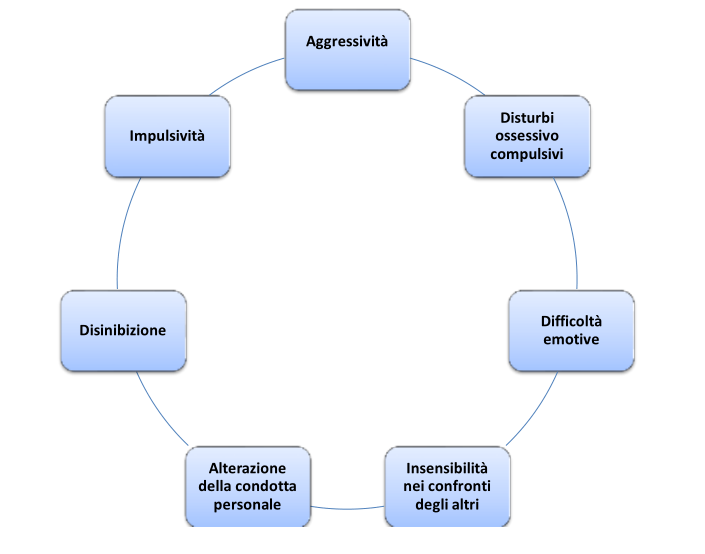
\includegraphics[width=\linewidth]{./images/image2}

\subsection{Basi neurali} 

\begin{itemize}
    \item Danni frontali
    \item Insula
    \item Cingolo
\end{itemize}
Fattori determinanti sono le caratteristiche premorbose.

\subsection{Modelli} 

\paragraph{Marcatore somatico}  Incapacità di apprendere emotivamente.
\paragraph{Reciprocità risposte sociali}  Non sono in grado di riconoscere le emozioni negative altrui, quindi non riescono ad adeguarsi al contesto
\paragraph{Teoria della mente}  Funziona bene per i sociopatici innati, spiega che sanno fare inferenze corrette sui pensieri e gli stati d'animo altrui ma gli manca la risposta emotiva

\section{Schizofrenia}

Kraeplin la individua per primo: \emph{dementia praecox};
Bleuler conia il termine schizofrenia.
\medskip\\  
\textbf{Due componenti:} 
\begin{enumerate}
    \item sintomi psicotici acuti  
    \item deficit cognitivi e funzionali stabili
\end{enumerate}
È importante il riconoscimento precoce della malattia.
\medskip\\   
\textbf{Sintomi positivi:}
\begin{itemize}
    \item Pensiero esterno
    \item Pensiero trasmissibile    
    \item Eco del pensiero  
    \item Furto del pensiero
    \item Allucinazioni uditive in terza e seconda persona
    \item Deliri di controllo
    \item Deliri di riferimento
    \item Deliri di persecuzione
\end{itemize}
\medskip 
\textbf{Sintomi negativi:}
\begin{itemize}
    \item Appiattimento affettivo
    \item Alogia
    \item Abulia
    \item Asocialità-Anedonia
\end{itemize}
\medskip
\textbf{Alterazioni cognitive:}
\begin{itemize}
    \item Memoria di lavoro
    \item Funzioni esecutive
\end{itemize}
Persistono anche in caso di trattamenti con farmaci e si riscontrano anche in pazienti premorbosi o parenti di  primo grado.

\subsection{Modelli}
\medskip
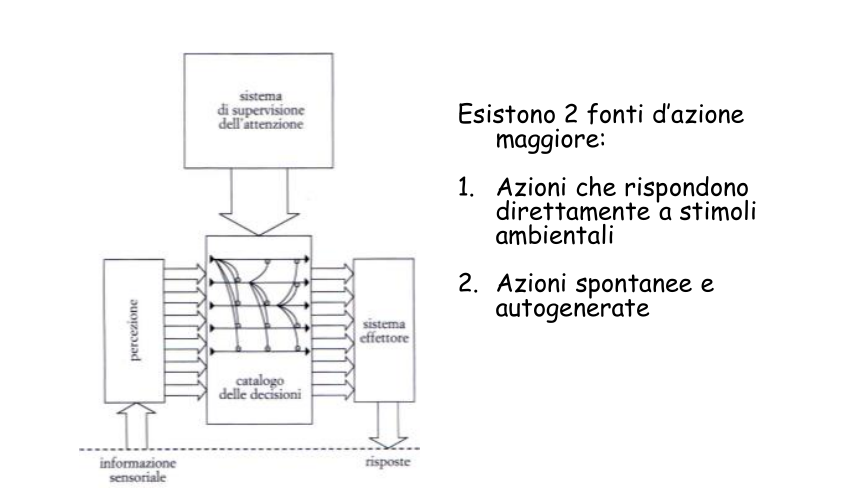
\includegraphics[width=\linewidth]{./images/image5}
\medskip\\
Un deficit nella produzione volontaria (sistema effettore) provoca i segni negativi, mentre i sintomi positivi avvengono perché il paziente attribuisce ad agenti esterni azioni e pensieri interni.

\paragraph{Modello del difetto dell'autocontrollo}  Gli schizofrenici non percepiscono la \textbf{scarica corollario}, ovvero lo sforzo di passare da un pensiero all'alt\-ro, e questo li fa sentire alieni ai propri pensieri.

\paragraph{Modello cognitivo unitario}  Difetti della metarappresentazione di sé e manca una teoria della mente per gli altri.

\paragraph{Determinismo multifattoriale}  Fattori biologici e genetici si uniscono a formare fragilità nei confronti della schizofrenia.

\subsection{Fattori biochimici} 

Sembra che la \textbf{dopamina} abbia relazioni importanti con la schizofrenia:
Un eccessivo rilascio (o quantità di recettori, o assenza di metabolizzatori) di dopamina nel sistema limbico è correlato con i sintomi positivi, mentre una diminuzione di dopamina nella corteccia meso-frontale potrebbe provocare i sintomi negativi.
\medskip\\ 
Anche un eccesso di serotonina sembra essere connessa con entrambi i sintomi.
\medskip\\ 
Infine l'anedonia potrebbe essere causata da un malfunzionamento del circuito della gratificazione, regolato dalla noradrenalina.

\subsection{Anomalie strutturali e funzionali} 

\paragraph{Allargamento ventricoli}  non è predittiva, si trova in molti disturbi.

\paragraph{Perdita materia grigia accelerata} durante l'adolescenza c'è un secondo sfoltimento delle sinapsi $\rightarrow$ la schizofrenia potrebbe derivare da un eccessivo sfoltimento.

\paragraph{Anomalie nell'ippocampo}  Riduzione volume, iperattività (molto importante nell'insorgenza del disturbo)

\paragraph{Brain derive neurotrophic factor}  è una proteina codificata dal gene BDNF e negli umani è presente prevalentemente a livello cerebrale. Promuove crescita e sviluppo e mantenimento dei neuroni e delle sinapsi, basse concentrazioni in schizo.
\medskip\\
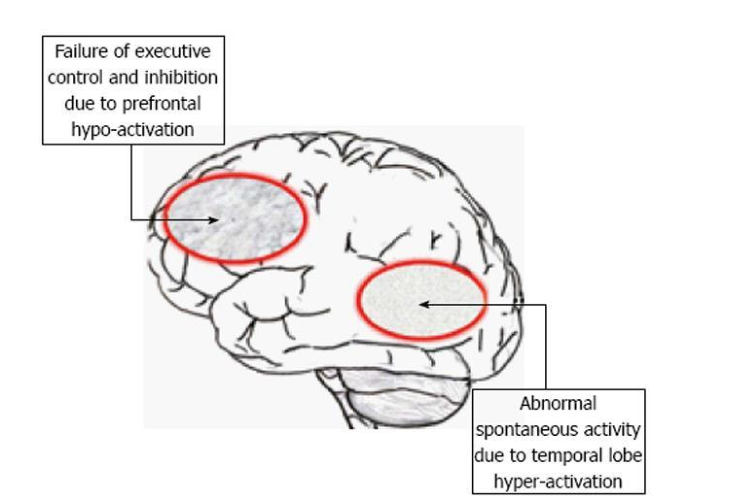
\includegraphics[width=\linewidth]{./images/image6}
\paragraph{Alterata connettività talamo, cervelletto e gangli}  potrebbe provocare movimenti bizzarri e smorfie.

\subsection{Fattori genetici} 

Alta ma non totale familiarità (50--70\% concordanza in monozigoti).\\
Rischio 10 volte maggiore per parenti.

\subsection{Fattori ambientali} 

La cultura influenza più che l'incidenza il decorso.\\
Schizofrenici più presenti in classi sociali basse (risultato più che causa)

\section{Depressione}

\subsection{Stress} 

Può essere provocato da fattori interni (frustrazione, mancata ricompensa attesa) o fisiologici (danni al corpo).
\medskip\\ 
Risposta aspecifica, legata alla sopravvivenza, solo inizialmente adattiva.
\paragraph{Risposta ormonale:} \emph{il cortisolo} \\ 
Gli agenti stressanti stimolano l'\textbf{ipotalamo}, attivando i \emph{nuclei paraventricolari} che producono \textbf{CRH} (corticotropin release hormone), che stimola l'\textbf{ipofisi} a produrre \textbf{ACTH} (ormone adrenocorticotropo) che agisce sulla zona corticale del surrene per produrre \textbf{cortisolo}. 
\medskip\\ 
Nel breve periodo il cortisolo ha un effetto di mobilitazione generale delle risorse dell'organismo mobilizzando le riserve energetiche.
\paragraph{Risposta nervosa:} l'autoregolazione di IIS\\
L'asse ipotalamo-ipofisi-surrene è autoregolantesi attraverso feedback negativo. Se questo non funziona bene $\rightarrow$ depressione.\\
\textbf{La depressione potrebbe essere dovuta ad un'attivazione cronica dell'asse IIS} 

\subsection{Effetti}

\begin{itemize}
    \item Asse della crescita
    \item Asse gonadico
    \item Asse tiroideo
\end{itemize}

\subsection{Psiconeuroimmunologia} 

Studia l'interazione tra fattori psichici, SNC e sistema immunitario.
Le \textbf{citochine} sono il medio comunicativo tra sistema immunitario e nervoso. Segnalano un danno, vengono recepite dall'ipotalamo, ipofisi, ecc\ldots
\medskip\\ 
IL-1 (interleuchina) è un tipo di citochina, attiva l'asse IIS\@.
Esiste anche l'interazione inversa, infatti le cellule del sistema immunitario hanno recettori per adrenalina, noradrenalina, cortisolo.

\subsection{Ipotesi monoaminergica} 

Viene scoperto casualmente che farmaci inibitori delle monoamine provocano attacchi depressivi e viceversa.
Vengono quindi utilizzati:
\begin{itemize}
    \item Inibitori MAO (monoaminossidasi): primi farmaci, molto efficaci ma con side effects
    \item Antidepressivi ciclici: inibiscono trasportatori noradrenalina e/o serotonina, efficaci ma effetti collaterali
    \item SSRI (inibitori selettivi della ricaptazione della serotonina): largo impi\-ego, pochi effetti collaterali.
\end{itemize}
In pratica si aumenta presenza monoamine.
L'effetto sui neurotrasmettitori è rapido ma la ripresa è lenta, questo è spiegato dalla lentezza della neurogenesi

\subsection{Anomalie funzionali} 

Ipoattivazione prefrontale sopratutto a sinistra

\section{Disturbi d'ansia}

\begin{itemize}
    \item Fobia specifica
    \item Disturbo d'ansia sociale
    \item Disturbo di panico 
    \item Agorafobia
    \item Disturbo d'ansia generalizzato
\end{itemize}

\subsection{Anomalie strutturali e funzionali} 

\begin{itemize}
    \item Iperattivazione amigdala
    \item Volume ippocampo ridotto, si attiva maggiormente
    \item Corteccia occipitale più attiva in risposta a stimoli minacciosi
    \item Talamo più attivo
\end{itemize}

\subsection{Anomalie biochimiche} 

\begin{itemize}
    \item \textbf{Sistema noradrenergico}: iperattivazione \emph{locus  coeruleus}, sembra implicato nella codifica dell'importanza degli stimoli. Genera iperattività mentale e ipercontrollo.
    \item \textbf{Sistema serotoninergico}: ipoattivazione nuclei del rafe, efficacia SSRI, ma LSD (serotoninergico) associato a insorgere disturbi d'ansia
    \item \textbf{GABA}: bassi livelli (sopratutto in amigdala) correlano con ansia. Le benzodiazepine (stimolano GABA) riducono l'ansia, ma creano dipendenza, sonnolenza e riducono capacità cognitive
    \item \textbf{Alterazione IIS}: aumentato rilascio di cortisolo
\end{itemize}

\subsection{Genetica} 

Possibile ruolo del gene che codifica il trasportatore della serotonina\\ (5HTTPLPR)

\subsection{Post-traumatic stress disorder} 

Frequenti immagini, evitamento di circostanze assimilabili al trauma, sovra eccitamento, ecc\ldots
\medskip\\ 
Ridotto controllo della corteccia su aree limbiche e cca, forse anche connessione potenziata tra amigdala e ipotalamo $\rightarrow$ sovrastimolazione IIS $\rightarrow$ \textbf{Ridotto volume ippocampo}
\medskip\\ 
Allele corto di 5HTTPLPR aumenta predisposizione

\subsection{Obsessive compulsive disorder} 

Non è più considerato un disturbo d'ansia, ci sono pensieri intrusivi.
\medskip\\ 
Malfunzionamento gangli della base (come in Tourette), quindi incapacità dell'orbitofrontale di inibire le risposte automatiche
\medskip\\  
Bassi livelli di serotonina e dopamina
\medskip\\ 
Sembra essere molto determinata geneticamente.
\medskip\\ 
Si tratta con Deep brain stimulation, farmaci o trattamento neurochirurgico, sembra che anche TMS funzioni.

\section{Sinestesia}

Misurabile attraverso
\begin{itemize}
    \item Stroop
    \item Esplorazione visiva
    \item Interferenza cross modale
\end{itemize}

\subsection{Modello} 

\paragraph{Teoria della sinestesia neonatale}:\\  
Pruning non completo nella prima infanzia

\paragraph{Teoria del feedback disinibito}:\\  
Aree contigue non abbastanza inibite

\paragraph{Cambiamenti di comunicazione con le aree associative}:\\
Aumento anomalo dell'integrazione grazie a iperattività delle regioni parietali (evidenza con studio tms)

\subsection{Ruolo dei fattori genetici} 

Congenita $\frac{1}{3}$ delle volte, più comune nelle donne, ma non si capace perché 

Può essere acquisita con uso di droghe o \textbf{deafferentazione} 

\section{L'invecchiamento}

Inizialmente \textbf{l'ipotesi della collina}: massimo adolescenziale di capacità cognitive, poi declino.

Poi \textbf{Life Spand Development Theory Psychology}: studi longitudinali, invecchiamento come interazione dinamica tra guadagni e perdite.

Due tipi di intelligenza:
\begin{itemize}
    \item Fluida: permette di adattarsi, declina da 25 anni in poi
    \item Cristallizzata: nozionistica, stabile fino ai 70
\end{itemize}

Due tipi di approcci:
\begin{itemize}
    \item Analitico/locale: studia i processi distinti che decadono con l'età, non permette di spiegare come né perché ciò avvenga
    \item Globale/macro: invecchiamento come modificazione nelle risorse mentali, e individua 3 risorse di elaborazione che decadono: 
        \begin{itemize}
            \item Memoria di lavoro
            \item Inibizione cognitiva
            \item Velocità di elaborazione
        \end{itemize}
\end{itemize}

Molti studi sulle capacità cognitive sono influenzati dal decadimento delle capacità sensoriali negli anziani.

\paragraph{Teoria dei processi automatici e controllati}  è una teoria globale, distingue tra processi \textbf{automatici e controllati} 

Uno dei processi più importanti che si deteriora è la \textbf{memoria di lavoro}, (e episodica dichiarativa e prospettica basata sul tempo anziché sugli eventi) per 3 possibili cause:
\begin{itemize}
    \item velocità di elaborazione ridotta
    \item deficit di inibizione
    \item declino differenziale (non abitudine a materiale visuospaziale es.\ computer)
\end{itemize}

\paragraph{Teoria della selettività socioemotiva}  nel tempo si presta più attenzione alla soddisfazione momentanea anziché  agli obbiettivi futuri, avendo tempo limitato.


Il \emph{reminiscence bump} è il fenomeno per il quale si è facilitati nella memoria autobiografica del periodo tra i 10 e i 30 anni.

\paragraph{Le funzioni esecutive}  updating shifting e inhibition declinano dopo i 60.

\subsection{Cambiamenti fisiologici} 

Cambiamenti nei circuiti fronto-striatali, sostanza bianca, grigia e dopamina ridotta nel frontale, meno volume nello striato.

\paragraph{Non c'è relazione tra danno cerebrale e manifestazioni cliniche:}  teoria della riserva cognitiva e cerebrale, dipende dalla quantità di conoscenze e circuiti possono compensare ai danni (the nun study)

La compensazione ha dei riscontri osservabili nella minore specializzazione emisferica nelle aree frontali in tarda età.

\subsection{La cura} 

Training metacognitivo: funziona meglio in anziani
\begin{itemize}
    \item Giovani
    \item Istruiti
    \item Con un buon vocabolario
    \item Non depressi
\end{itemize}

\subsection{Demenze} 
    
\paragraph{Alzheimer}:\\
Deficit: 
\begin{itemize}
    \item memoria episodica 
    \item linguaggio
    \item abilità visuo-spaziali
    \item percezione
    \item prassia
    \item funzioni esecutive
\end{itemize}
Alterazioni:
\begin{itemize}
    \item Strutture temporali mediali (ippocampo e entorinale)
    \item Cortecce associative  
    \item Corteccia prefrontale
\end{itemize}
Patogenesi:\\
Accumulo $\beta$-amiloide, teoria della cascata del $\beta$-amiloide:

I peptidi A$\beta$ sono frammenti proteici prodotti dalla scissione di una proteina maggiore (precursore dell'amiloide), componente della membrana cellulare. L'A$\beta$42 è più suscettibile ad aggregarsi in ammassi insolubili, dette **placche amiloidi**, sottili filamenti che si formano nello spazio extracellulare, nella parte centrale costituiti da A$\beta$, e nella parte periferica detri\-ti neuronali (frammenti assonali).Questo accumulo provocherebbe una casca\-ta di alterazioni
della **proteina tau**, una famiglia di proteine utiliz\-zate per l'assemblaggio dei microtuboli (strutture del citoscheletro responsa\-bili del trasporto di molecole all'interno  degli assoni delle cellule nervose). Una forma iperfosforilata della tau, compromette il trasporto assonale e quindi causa la morte cellulare.
\medskip\\
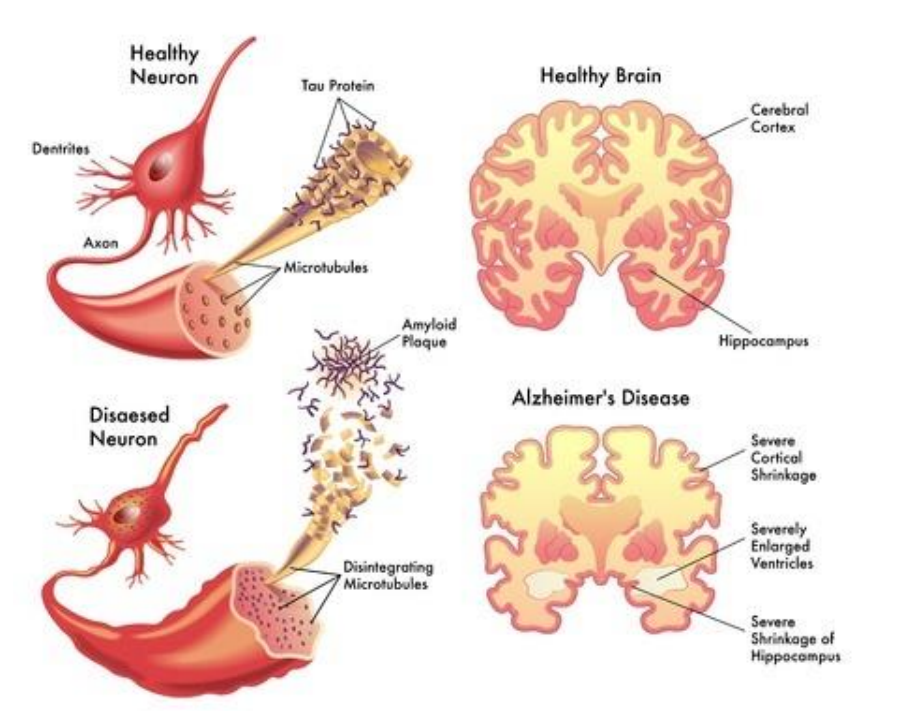
\includegraphics[width=\linewidth]{./images/image8}
\medskip\\
Biomarkers:
\begin{itemize}
    \item Placche amiloidi, 10-15 anni prima dell'esordio clinico
    \item Neurodegenerazione e danni neuronali, positivi successivamente
\end{itemize}
\paragraph{Mild Cognitive Impairment}  MCI 

Punteggi nei test cognitivi sotto la media, ma ancora non condizione clinica, ma la predice. Può durare anche 10 anni, c'è ottima correlazione anatomo-patologica (alterazioni entorinali e ippocampali)







\end{document}
